\section{Regression}

In this first part we are gonna focus on fitting lines to datapoints. For this we will introduce the \textbf{machine learning pipeline}. It consists of three parts and has the goal to find the optimal model $\hat{f}$ for given data $D$, that we can use to predict new data.

\smallskip
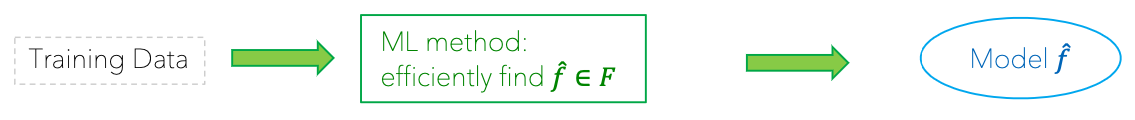
\includegraphics[width=\columnwidth]{ml-pipeline.png}

The three parts of the ML Pipeline are the function class $\mathbf{F}$, the loss function $\ell$ and the optimization method. \medskip

In the coming sections $f^*$ will be the ground truth function and $\hat f$ will be used for our (learned) prediction model.

\subsection{Linear Regression}

Given the data $(x_i, y_i)$ we use models of the form $f(x) = w^\top x + b$ to fit the data. To find the optimal values for $w$ and $b$ we try to reduce the \textbf{squared loss}:
$$\ell(y, f(x)) := \frac{1}{n}\sum (y_i - f(x_i))^2 = \frac{1}{n}||y - X w||_2^2$$

In the matrix notation $b$ is part of $w$. The closed form solution for linear regression is given by the normal equation $Ax - b \Rightarrow x = (A^\top A)^{-1} A^\top y$:
$$\hat{w} = (X^\top X)^{-1}X^\top y$$

\columnbreak

We can also get the closed form solution by using the fact that the squared loss is a convex function and $\hat{w}$ is the global minima of this function. Therefore we can calculate the gradient $\nabla \ell(y, f(x))$ and solve for $0$ to find $\hat{w}$. Later, we will see a more efficient way of finding $\hat{w}$. \medskip

\subsubsection{Different Loss Functions}

The square loss penalizes over- and underestimation the same. Further it puts a large penalty on outliers (grows quadratically). While this is often good, we might want a different loss function, some possibilities are:

\begin{itemize}
	\item Huber loss - ignores outliers ($a = y - f(x)$
		$$\ell_\delta(y, f(x)) := \begin{cases}
			\frac{1}{2} a^2 & \text{for } |a| \leq \delta \\
			\delta \cdot (|a| - \frac{1}{2} \cdot \delta) & \text{otherwise}
		\end{cases}$$
	\item Asymmetric losses - weigh over- and underestimation differently
\end{itemize}

\subsection{Nonlinear Functions}

Linear functions helped us to keep the calculations "simple" and find good solutions. But often there are problems that are more complex and would require nonlinear functions. The avoid using nonlinear functions we introduce feature mapping. 

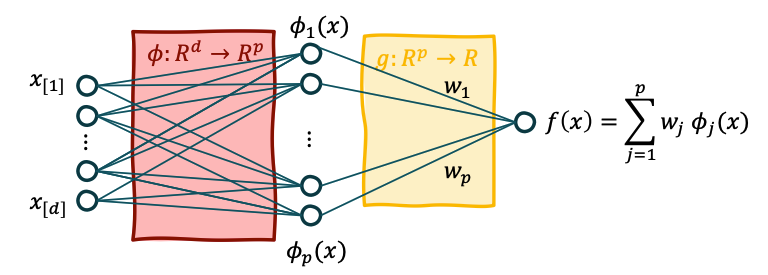
\includegraphics[width=\columnwidth]{feature-mapping.png}

From our input vector $x$ we extract a \textbf{feature vector} $\phi(x)$ by using a fixed mapping $\phi$ that can consist of any nonlinear function. On this feature vector we can use the already known methods for linear functions to find a solution.

\subsection{Regularization}

We will later see that too complex models are not always good, as they use too many features. If we want to reduce the number of features, we can encourage sparsity by introducing a penalty term. 

We commonly use:
\begin{itemize}
	\item \textbf{Lasso Regression}: $\argmin{w \in \R^d} ||y - \Phi w||^2 + \lambda ||w||_1$
	\item \textbf{Ridge Regression}: $\argmin{w \in \R^d} ||y - \Phi w||^2 + \lambda ||w||_2$
\end{itemize}

Lasso regression sets a lot of weights to zero, while ridge regression just puts the focus on lower weights.